\chapter{Otros sistemas oscilantes}

\vspace{-5mm}%***********************************************
\begin{miparrafo}
	\small{Al observar la Naturaleza nos damos cuenta de que muchos procesos físicos (por ejemplo la rotación de la tierra en torno al eje polar) son repetitivos, sucediéndose los hechos cíclicamente tras un intervalo de tiempo fijo. En estos casos hablamos de movimiento periódico y lo caracterizamos mediante su período, que es el tiempo necesario para un ciclo completo del movimiento, o su frecuencia, que representa el número de ciclos completos por unidad de tiempo.}

\small{Un caso interesante de movimiento periódico aparece cuando un sistema físico oscila alrededor de una posición de equilibrio estable. El sistema realiza la misma trayectoria, primero en un sentido y después en el sentido opuesto, invirtiendo el sentido de su movimiento en los dos extremos de la trayectoria. Un ciclo completo incluye atravesar dos veces la posición de equilibrio. La masa sujeta al extremo de un péndulo o de un resorte, la carga eléctrica almacenada en un condensador, las cuerdas de un instrumento musical, y las moléculas de una red cristalina son ejemplos de sistemas físicos que a menudo realizan movimiento oscilatorio.}

\small{El caso más sencillo de movimiento oscilatorio se denomina movimiento armónico simple y se produce cuando la fuerza resultante que actúa sobre el sistema es una fuerza restauradora lineal. El Teorema de Fourier nos da una razón de la importancia del movimiento armónico simple. Según este teorema, cualquier clase de movimiento periódico u oscilatorio puede considerarse como la suma de movimientos armónicos simples}\normalsize{.}
\end{miparrafo}

\vspace{15mm} %***************************************************
\section{Oscilaciones armónicas}

Características el MAS: $\qquad F=-kx;\qquad \mathcal E_p=\dfrac 1 2 k x^2$

Movimiento vibratorio: un cuerpo o una partícula se mueve sucesivamente de un lado a otro de una posición de equilibrio, repitiendo a intervalos de tiempo regulares sus variables cinemáticas (posición, velocidad y aceleración).Cuando las oscilaciones son muy rápidas se denominan vibraciones y el movimiento correspondiente es un movimiento vibratorio

En movimiento vibratorio, llamando $x_0$ al punto de equilibrio, se tiene:
$F=-k(x-x_0); \qquad \mathcal E_p=\dfrac 1 2 k (x-x_0)^2$

\begin{multicols}{2}
$\quad$ 

La representación gráfica $\mathcal E_p - x$ en forma de parábola es característica del movimiento vibratorio. La parábola es simétrica respecto de $x_0$ en que presenta un mínimos, por el teorema de Lejeune Dirichlet (ver seccción \ref{Lejeune-Dirichlet}) en $x_0$ hay un mínimo por lo que el equilibrio es estable.

\begin{figure}[H]
		\centering
		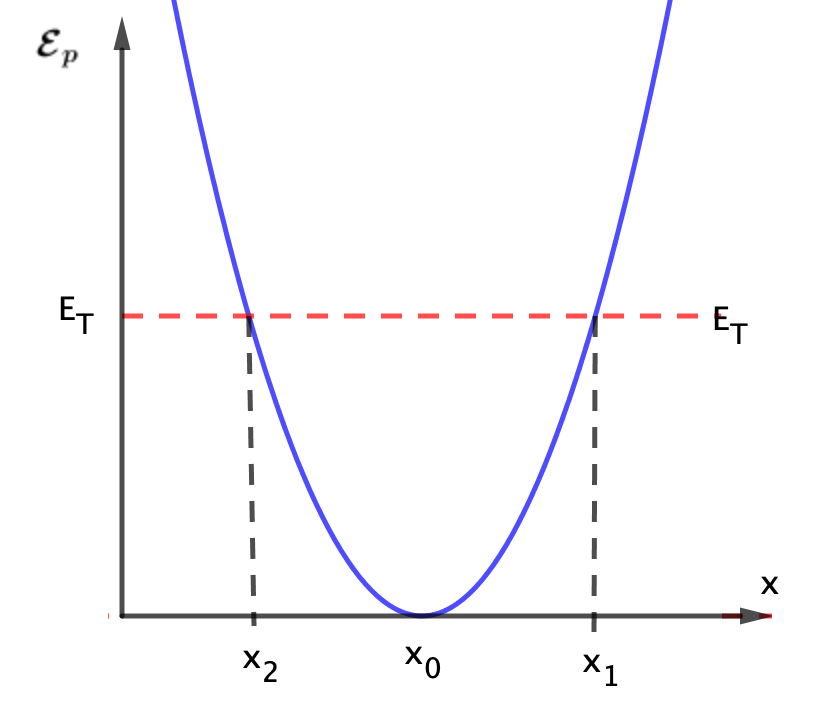
\includegraphics[width=.35\textwidth]{imagenes/imagenes20/T20IM01.png}
	\end{figure}
\end{multicols}

\begin{multicols}{2}
En física hay otro tipo de movimientos vibratorios en los que la representación de la energía potencial no es una parábola pero sí tiene bien definido un mínimo en el punto de equilibrio.

Por consideraciones energéticas, el sistema oscila entre $x_2$ y $x_2$.

Este tipo de oscilaciones se las conoce con el nombre de \emph{oscilaciones anarmónicas}.
\begin{figure}[H]
		\centering
		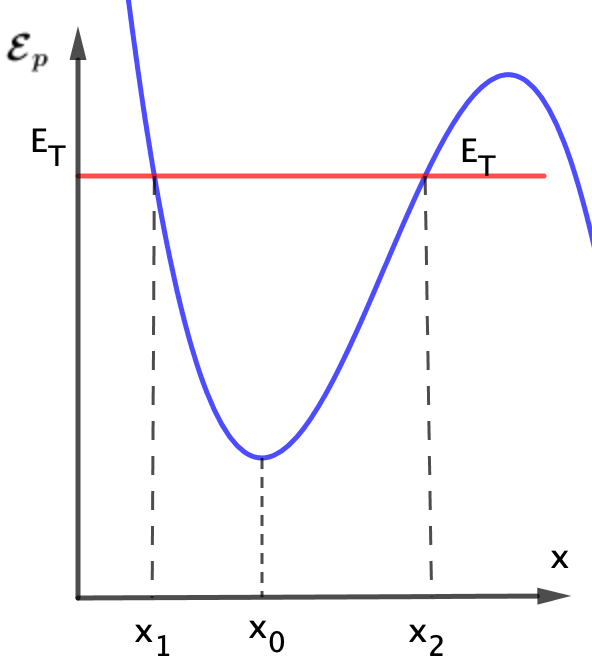
\includegraphics[width=.3\textwidth]{imagenes/imagenes20/T20IM02.png}
	\end{figure}
\end{multicols}

La energía potencial será función de la posición, pero no del tiempo (no estaríamos tratando con campos conservativos) $\ \mathcal E_p=\mathcal E_p(x)$.

Experimentalmente sabemos que $a)$ la partícula oscila y $b)$ lo hace alrededor de una posición de equilibrio.

Establcemos la hipótesis matemática de que la función de la energía potencial en función de la posición que ocupa la partícula es \emph{continua}, por Taylor\footnote{Ver apéndice \ref{McLaurin}}:

$\displaystyle \mathcal E_p(x)=\mathcal E_p(x_0)+\left(\dv{\mathcal E_p}{x}\right)_{x_0}(x-x_0)+ \dfrac 1{2!}\left(\dv[2]{\mathcal E_p}{x}\right)_{x_0}(x-x_0)^2$

$\displaystyle +\dfrac 1{3!}\left(\dv[3]{\mathcal E_p}{x}\right)_{x_0}(x-x_0)^3+\cdots$

$\mathcal E_p(x_0)$ es la constante arbitraria de la energía potencial, la neregía potencial en el punto de equilibrio.

Como $x_0$ es un mínimo, $\displaystyle \left(\dv{\mathcal E_p}{x}\right)_{x_0}=0$ y además $\displaystyle \left(\dv[2]{\mathcal E_p}{x}\right)_{x_0}=k>0$, por el mismo motivo.

Por todo ello: $\displaystyle \mathcal E_p(x)=\mathcal E_p(x_0)+ \dfrac 1{2!} k(x-x_0)^2 +\dfrac 1 {3!} k' (x-x_0)^3 + \cdots$

En el MAS: $\displaystyle \mathcal E_p=\dfrac 1 2 k (x-x_0)^2 \to \dv{\mathcal E_p}{x}=k(x-x_0) \to \dv[2]{\mathcal E_p}{x}=k=cte$ elástica o de recuperación de la fuerza. 

Es por analogía con el más que hemos llamado, más arriba, $k=\displaystyle \left(\dv[2]{\mathcal E_p}{x}\right)_{x_0}$, pero no por otra cosa.

Suponemos que estamos estudiando un caso particular para el cual la energía mecánica $E_T$ sea lo suficientemente pequeña para que $(x-x_0)^2<<(x-x_0)$; en estas condiciones:
$\ \displaystyle \mathcal E_p \approx \mathcal E_p(x_0)+\dfrac 1 2 k (x-x_0)^2$

La energía potencial estará constituida por dos partes, una constante y una función oscilador armónico simple.

Calculando ahora la fuerza:  $\ F=-\displaystyle \dv{\mathcal E_p}{x}=-K(x-x_0)$

Toda partícula que oscila sobre un valor de equilibrio presenta un mínimo en ese punto de equilibrio.

Si los resultados no coinciden con la experiencia es porque hay que considerar más términos del desarrollo de Taylor de la energía potencial.

\section{Oscilaciones amortiguadas}

En la naturaleza, los movimientos oscilatorios no existen. Van perdiendo amplitud paulatinamente hasta que se detienen.

Vamos a ver, para una dimensión, el caso de que las fuerzas de rozamiento hacen que el cuerpo oscilante se pare.

$F_T=F_e+F_m$; $\ F_e$ es la fuerza elástica ($-kx$) y $F_m$ la fuerza del medio (de rozamiento). Experimentalmente se comprueba que las fuerzas de medio son proporcionales a una determinada potencia de la velocidad, en esta caso supondremos que dependen de la primera potencia de la velocidad: $F_m=-bv$ (negativa, pues se opone al movimiento).

Segunda de Newton:  $\ F_T=ma=-Kx-bv$, luego

$$\subrayado{\ \displaystyle m\ \dv[2]{x}{t}\ +\ b\ \dv{x}{t}+kx\ = \ 0 \ }$$

ecuación diferencial lineal homogénea de segundo orden.\footnote{Para más información, ver apéndice \ref{EDO}.}

Ecuación característica: $\ mp^2+bp+k=0 \to p=-\dfrac {b}{2m} \pm \left[ \left( \dfrac {b}{2m} \right)^2 - \left( \dfrac k m \right) \right]^{1/2}$

Llamamos $\gamma=\dfrac {b}{2m}$, \emph{coeficiente de amortiguamiento} y $\omega^2=\dfrac{k}{m}$, que en el caso del oscilador armónico es la frecuencia angular.

Las soluciones de la ecuación característica son, ahora, $p=-\gamma \pm \sqrt{\gamma^2-\omega^2}$

Vamos a estudiar tres casos:

\begin{itemize}
\item $\gamma < \omega \qquad$ (raíces $p$ imaginarias - \emph{infraamortiguado})

$(\gamma^2-\omega^2)^{1/2}=i(\omega^2-\gamma^2)^{1/2}=\pm i \omega_1 \to p=-\gamma \pm i \omega_1$

\begin{multicols}{2}
La solución general es estos casos es: $\quad x=Ae^{-\gamma t}\cos(\omega_1t+\alpha)$

$A e^{-\gamma t}$ es la amplitud instantánea. Se trata del tipo de movimiento del péndulo simple.
\begin{figure}[H]
		\centering
		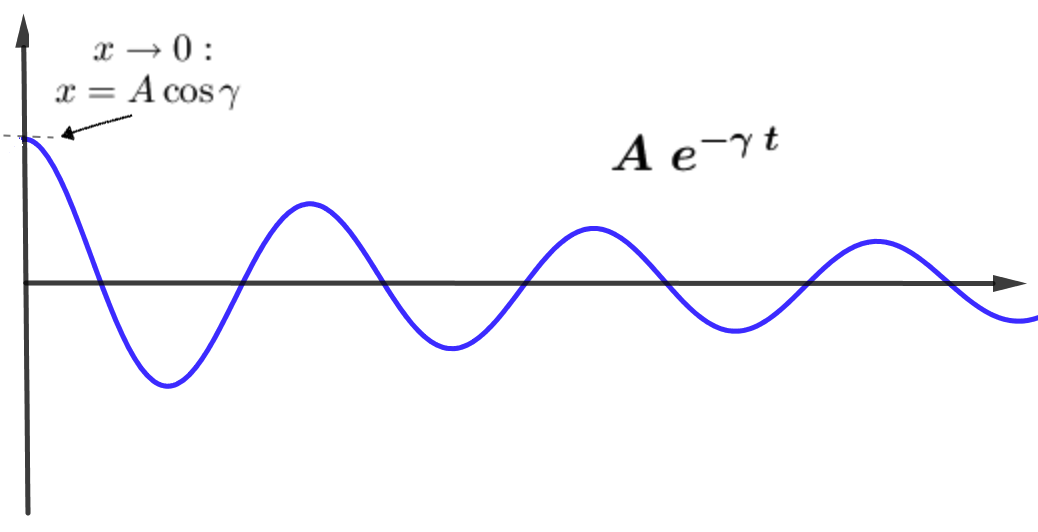
\includegraphics[width=.5\textwidth]{imagenes/imagenes20/T20IM03.png}
	\end{figure}
\end{multicols}

\item $\gamma > \omega \qquad$ (raíces $p$ reales y distintas - \emph{sobreamortiguado})

$p_1=-\gamma + (\gamma^2-\omega^2)^{1/2}=-\gamma_1; \quad
p_2=-\gamma - (\gamma^2-\omega^2)^{1/2}=-\gamma_2 $

La solución más general es: $x=Ae^{-\gamma_1 t}+Be^{-\gamma_2 t}$

\begin{multicols}{2}
Exponenciales decrecientes; en este caso, la amplitud decae más rápidamente que en el anterior.

Es el caso de un péndulo muy ligero oscilando sumergido en agua.
\begin{figure}[H]
		\centering
		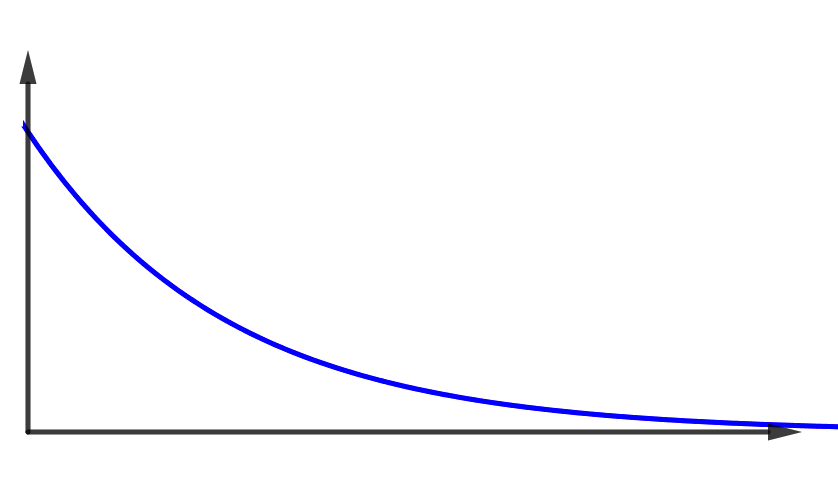
\includegraphics[width=.5\textwidth]{imagenes/imagenes20/T20IM04.png}
	\end{figure}
\end{multicols}
\item $\gamma = \omega \qquad$	($p$ es una raíz real doble - \emph{amortiguamiento crítico})

$p=-\gamma = \to x=(A+Bt)e^{-\gamma t}$

El amortiguamiento crítico proporciona la forma más rápida de aproximar a cero la amplitud de un oscilador amortiguado. Con menor amortiguamiento (subamortiguación) alcanza el cero más rápidamente, pero oscila alrededor de él. Con mas amortiguamiento (sobreamortiguación), el acercamiento a cero es más lento. La amortiguación crítica, ocurre cuando el coeficiente de amortiguación es igual a la frecuencia de resonancia sin amortiguación del oscilador.
\end{itemize}

\begin{figure}[H]
		\centering
		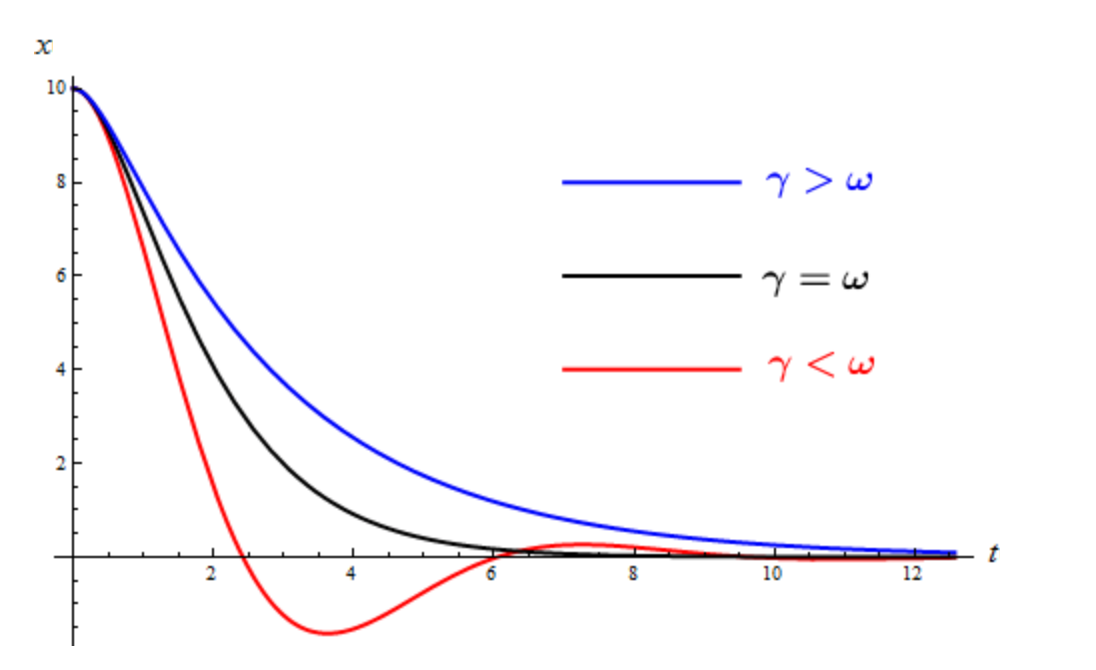
\includegraphics[width=.95\textwidth]{imagenes/imagenes20/T20IM06.png}
	\end{figure}

\section[Oscilaciones forzadas. Resonancia. Transmisión de energía]{Oscilaciones forzadas. Resonancia. Transmisión de energía\sectionmark{Oscilaciones forzadas}}
\sectionmark{Oscilaciones forzadas}

Vamos a estudiar el caso en el que sobre nuestro oscilador actúa, además de la fuerza elástica ($F_e=-kx$) y la fuerza del medio ($f_m=-bv$) otra fuerza esta vez periódica $F_p=F\cos \omega t$).

Segunda de Newton: $F_t=\displaystyle ma=-kx-bv+F\cos \omega t$

$$\subrayado{\ \displaystyle m\ \dv[2]{x}{t}\ +\ b\ \dv{x}{t}+kx\ = \ F\cos \omega t \ }$$

ecuación diferencial lineal \emph{completa} de segundo orden.

La solución más general consta de la solución de la homogénea, $x_h$, más una solución particular, $x_i$: $\quad x=x_h+x_i$

$x_h=Ae^{-\gamma t}\cos (\omega_1t+\varphi)$, con $\omega_1=(\omega_0^2-\gamma^2)^{1/2} \text{ y } \gamma=\dfrac{b}{2m}$; $\ \omega_0=\sqrt{\dfrac k m}$, frecuencia propia del oscilador.

$x_i=p\cos \omega t + q \sin \omega t$. En este caso, $\omega$ es la frecuencia externa de la fuerza periódica. $p \text{ y } q$ son cosntantes a determinar por las condiciones físicas del problema ($m, b, x, F, \cdots)$).

Sustituiremos la  $x_i$ por la $x$ de la ecuación diferencial de segundo orden e identificaremos los coeficientes en senos y cosenos de ambos miembros.

$\displaystyle \dv{x_i}{t}=-p\omega \sin \omega t +q\omega
\cos \omega t; \qquad \displaystyle \dv[2]{x_i}{t}=-p\omega^2 \cos \omega t - q \omega^2 \sin \omega t$

$-mp\omega^2 \cos \omega t-mq\omega^2 \sin \omega t -bp\omega \sin \omega t +bq\omega \cos \omega t +kp\cos \omega t +kq\sin \omega t=F\cos \omega t$

Identificando: $\quad \begin{cases}
 \ \ (k-m\omega^2)p+b\omega q=F \\ -b\omega p+(k-m\omega^2)q=0	
 \end{cases}$
 
 Dos ecuaciones con dos incógnitas: $\quad \begin{cases}
\ \ p=\dfrac{F(k-m\omega^2)}{(k-m\omega^2)^2+b^2\omega^2} \\ \ \ q=\dfrac{Fb\omega)}{\sqrt{(k-m\omega^2)^2+b^2\omega^2}}	
\end{cases}$

Llevando estos resultados a $x_i=p\cos \omega t + q \sin \omega t \ \to$

\small{$x_i=\dfrac{F}{\sqrt{(k-m\omega^2)^2+b^2\omega^2}} \left[
\dfrac{(k-m\omega^2)}{\sqrt{(k-m\omega^2)^2+b^2\omega^2}}+
\dfrac{b\omega}{\sqrt{(k-m\omega^2)^2+b^2\omega^2}}\sin \omega t
\right]=$}

\normalsize{$\dfrac{F}{\sqrt{(k-m\omega^2)^2+b^2\omega^2}} [A+B\sin \omega t]$}

Llamando $\cos \alpha=A;\ \ \sin \alpha =B \ \to \ \text{Pitágoras} \ \ A^2+B^2=1$ y teniendo en cuenta el desarrollo en serie de potencias de McLaurin del $\sin (\omega t + \alpha)$, \textcolor{gris}{$\cos \alpha=\dfrac{(k-m\omega^2)}{\sqrt{(k-m\omega^2)^2+b^2\omega^2}}$} y \textcolor{gris}{$\sin \alpha=\dfrac{b\omega}{\sqrt{(k-m\omega^2)^2+b^2\omega^2}}\sin \omega t\ $} podremos escribir.

$x_i=\dfrac{F}{\sqrt{(k-m\omega^2)^2+b^2\omega^2}} \sin (\omega t + \alpha)$

Como $\sqrt{(k-m\omega^2)^2+b^2\omega^2}=cte=G$ y como $\tan \alpha= \dfrac{k-m\omega^2}{b\omega} \ \to \  x_i=\dfrac F G \sin (\omega t +\alpha ) = C  \sin (\omega t +\alpha ) \qquad C=\dfrac F G$

La solución general es:

$$ \subrayado{ \ x= A\ e^{-\gamma t} \ \cos (\omega_1t+ \varphi) \ + \ C \ \sin (\omega t + \alpha) \ } $$

Analizando la solución general, aparecen dos términos: el primero corresponde a ondas que se amortiguan (caen muy deprisa) y el segundo corresponde al MAS.

Para un determinado tiempo en que el primer término ya haya caído, $\tau$, solo queda el segundo término, $x=C\sin(\omega t + \alpha),\quad t\leq \tau$

$A\ e^{-\gamma t} \ \cos (\omega_1t+ \varphi) \ $ es la \emph{solución transitoria}; $C \ \sin (\omega t + \alpha) \ $ es la \emph{solución estacionaria}.

Trabajemos con la solución estacionaria y vemos que el sistema vibra con la misma frecuencia $\omega$ de la fuerza periódica: $x=A \sin (\omega t + \alpha) $
con $A=\dfrac F G= \dfrac A {\sqrt{m^2(\omega_0^2-\omega^2)^2+b^2\omega^2}}$ y $\tan \alpha=\dfrac{\omega_0^2- \omega^2}{\frac b m \omega^2}$

\begin{multicols}{2}
Representación de la amplitud $A$ del movimiento resultante en función de la frecuencia propia $\omega$ 
$\omega_A$ se obtiene derivando, $\displaystyle \dv{A}{\omega}=0$, se obtiene: $\ \omega_A=\sqrt{\omega_0^2-\left( \dfrac{b}{\sqrt{2m}} \right)^2}$
\begin{figure}[H]
		\centering
		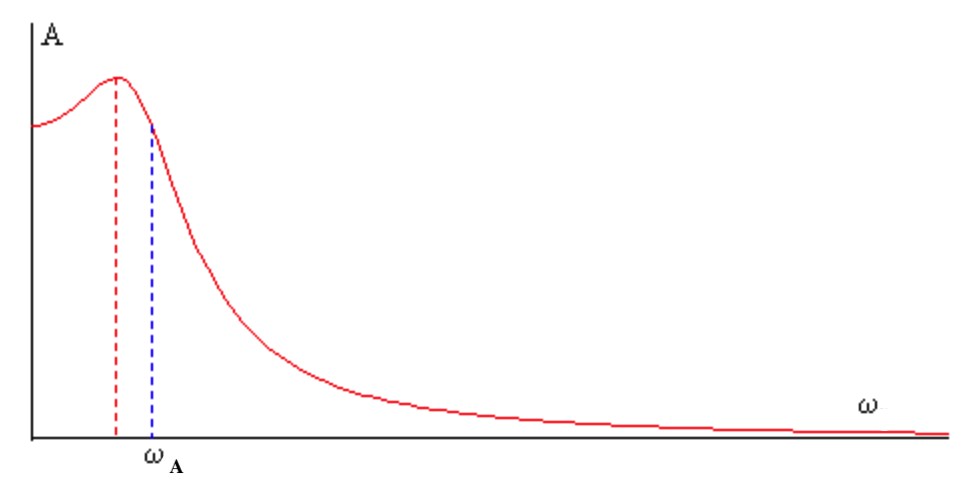
\includegraphics[width=.4\textwidth]{imagenes/imagenes20/T20IM07.png}
	\end{figure}	
\end{multicols}

A esta frecuencia para la cual la amplitud del sistema es máxima dados un medio $b$ y una fuerza periódica $F$ se le conoce con el nombre de \emph{frecuencia de resonancia en amplitud}.

Representemos $A$ frente a $\omega$ para distintos valores de $b$

Para $b=0$ y $\omega=\omega_0$, en la ecuación de $A=\frac F G$, el denominador tiende a cero y el valor de la amplitud se dispara a infinito.

\vspace{10mm} %****************************************
\begin{figure}[H]
		\centering
		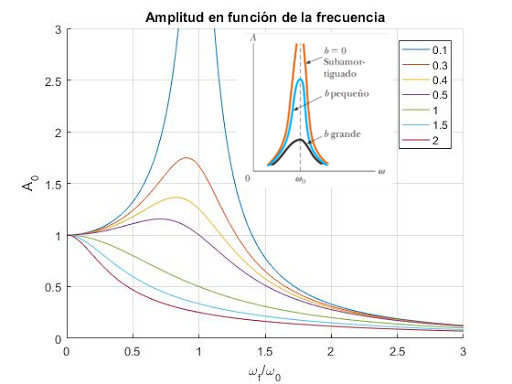
\includegraphics[width=.8\textwidth]{imagenes/imagenes20/T20IM08.png}
\end{figure}	
\vspace{10mm} %****************************************
Para un oscilador dado, a medida que $b$ crece, $\omega_A$ se va haciendo más pequeño lo que significa que el máximo se desplaza hacia la izquierda.

$\omega_1=\sqrt{\omega_0^2-\left( \dfrac b{2m} \right)^2}$. \hspace{5mm} Se verifica que: $\omega_0>\omega_1>\omega_A$

Vamos ahora a calcular la velocidad con que se mueve el sistema que tiene asociada una fuerza periódica.

$\displaystyle v=\dv{x}{t}=\omega t \cos(\omega t + \alpha); \qquad F(t)=F\cos \omega t$

Podemos interpretar $\alpha$ como el desfase entre la velocidad y la fuerza aplicada.

\vspace{30mm} %****************************************
\begin{multicols}{2}
En módulo, 

$\ v_0=\omega A=\dfrac{F}{\sqrt{m^2 \left( \dfrac{\omega_0^2}{\omega}-\omega \right)^2+b^2}} \ \to \ v_0=v_0(\omega)$

El módulo de la velocidad es función de la frecuencia que acompaña a la fuerza aplicada. Representando $v_0$ frente a $\omega$.

\begin{figure}[H]
		\centering
		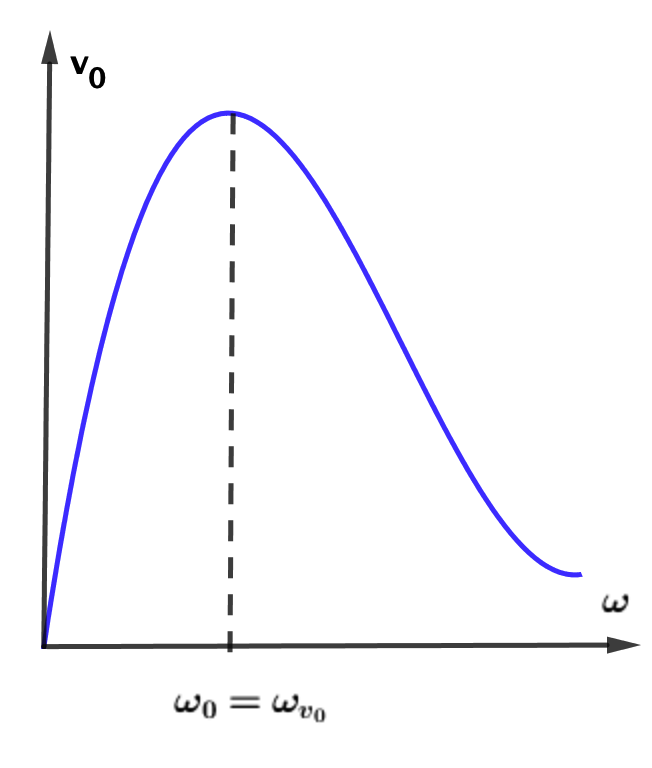
\includegraphics[width=.25\textwidth]{imagenes/imagenes20/T20IM09.png}
	\end{figure}	
\end{multicols}
Para que $v_0$ sea máximo, $\boldsymbol{ \omega_{v_0}=\omega_0 }$. Para este valor de $\omega_0$, el oscilador gira con $A$ máxima $\to \alpha=0$, la velocidad del movimiento y la fuerza aplicada están en fase: \emph{condición de resonancia en la velocidad.}

Veamos cuales son las condiciones de resonancia en la energía:

Potencia, $\ \mathcal P=\displaystyle \dv{E}{t}=F(t)v(t)$. La condición experimental es $F(t)$ y $v(t)$ es la respuesta del sistema.

El valor máximo que tomará la potencia será aquel para el cual en unas condiciones determinadas el producto $F$ por $v$ sea máximo. La respuesta del sistema será máxima cuando se cumplan las condiciones de resonancia de la velocidad, la potencia será máxima.

Cuando hay resonancia en la energía, la transferencia energética de la fuerza aplicada al oscilador forzado es máxima.

Si el oscilador está en un medio en que $b$ es muy pequeño, $\omega_0, \ \omega_A, \ \omega_{v_0}$ son prácticamente iguales.

En estas condiciones, el agente impulsor del oscilador transmite máxima amplitud y máxima energía al sistema.


\section[Análisis de Fourrier del movimiento periódico. Teorema de Fourrier]{Análisis de Fourrier del movimiento periódico. Teorema de Fourrier\sectionmark{Análisis de Fourrier}}
\sectionmark{Análisis de Fourrier}

Sea $f(t)=f(t+T)$ una función periódica.
\begin{figure}[H]
		\centering
		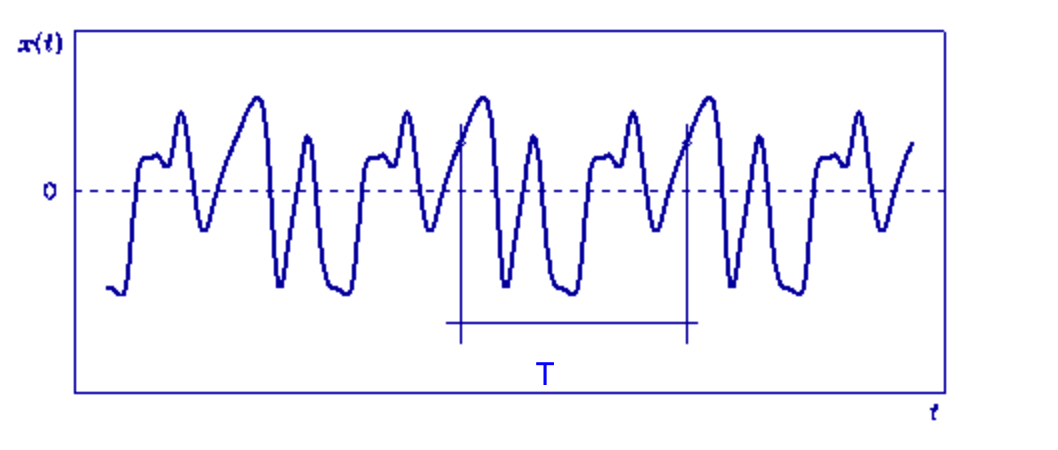
\includegraphics[width=.75\textwidth]{imagenes/imagenes20/T20IM10.png}
	\end{figure}	

\begin{teor}{Teorema de Fourrier}
Todo movimiento periódico se puede descomponer como suma de movimientos vibratorios armónicos de frecuencias múltiplos de la del movimiento periódico considerado, que se llama frecuencia fundamental.	
\end{teor}

$f(t)=a_0+a_1\cos \omega t +a_2\cos 2\omega t +a_3\cos 3\omega t + \cdots + b_1\sin \omega t +b_2\sin 2\omega t  + \cdots$

donde: 
\begin{table}[H]
%\centering
\begin{tabular}{l}
$\qquad a_0=\displaystyle \dfrac 1 T \int_0^T f(t) \ \dd t$ \\
$\qquad a_n=\displaystyle \dfrac 1 T \int_0^T f(t) \cos n\omega t \  \dd t$ \\
$\qquad b_n=\displaystyle \dfrac 1 T \int_0^T f(t) \sin n\omega t \ \dd t$
\end{tabular}
\end{table}

Admitido el teorema de Fourrier, procedemos a integrar $f(t)$ desde $0$ hasta $T$:

\hspace{-5mm}\small{$\displaystyle \int_0^T f(t)\ \dd t= a_0 \cancelto{T}{\int_0^T \dd T} + a_1 \cancelto{0}{\int_0^T \cos \omega t \ \dd t}+ \cdots + b_1\cancelto{0}{\int_0^T \sin \omega t \ \dd t}+ \cdots =a_0T$}

\normalsize{Despejando, obtenemos:} $\ a_0=\displaystyle \dfrac 1 T \int_0^T f(t)\ \dd t$

\begin{figure}[H]
		\centering
		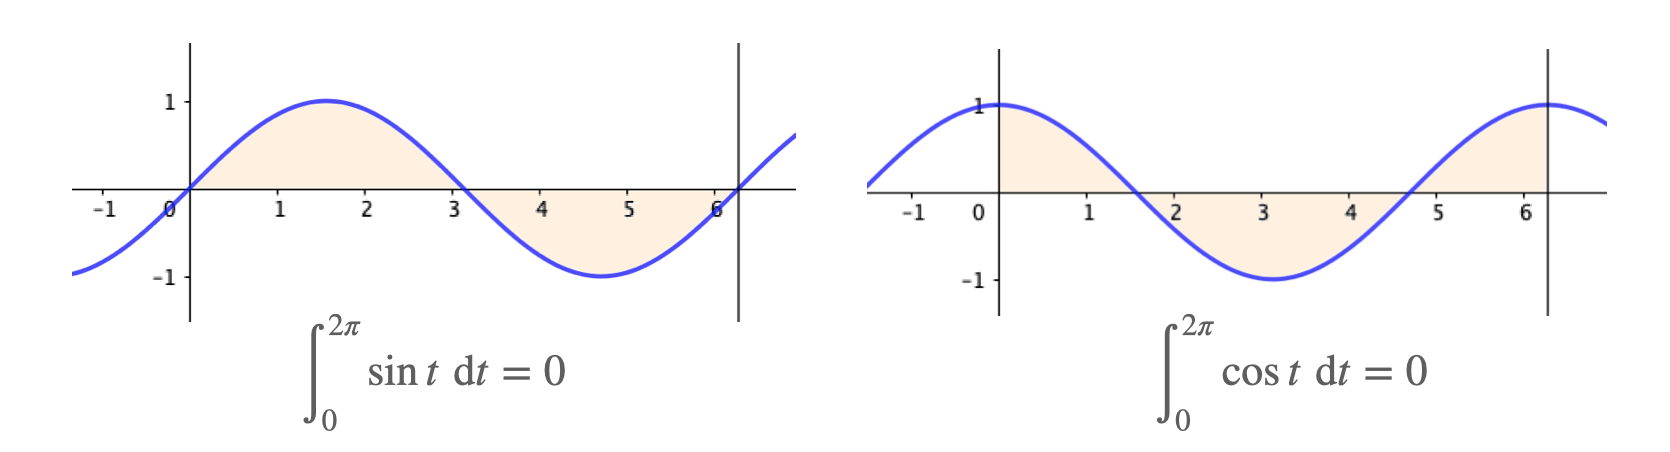
\includegraphics[width=1\textwidth]{imagenes/imagenes20/T20IM11.png}
	\end{figure}

\newpage
\begin{myblock}{Análisis de Fourrier}
Una serie de Fourier es una serie infinita que converge puntualmente a una función periódica y continua a trozos (o por partes). Las series de Fourier constituyen la herramienta matemática básica del análisis de Fourier empleado para analizar funciones periódicas a través de la descomposición de dicha función en una suma infinita de funciones sinusoidales mucho más simples (como combinación de senos y cosenos con frecuencias enteras). 
%\begin{multicols}{2}

\vspace{2mm} El nombre se debe al matemático francés Jean-Baptiste Joseph Fourier, que desarrolló la teoría cuando estudiaba la ecuación del calor. Fue el primero que estudió tales series sistemáticamente, y publicó sus resultados iniciales en 1807 y 1811. Esta área de investigación se llama algunas veces análisis armónico.

\vspace{2mm} Es una aplicación usada en muchas ramas de la ingeniería, además de ser una herramienta sumamente útil en la teoría matemática abstracta. Sus áreas de aplicación incluyen análisis vibratorio, acústica, óptica, procesamiento de imágenes y señales, y compresión de datos.


\begin{figure}[H]
		\centering
		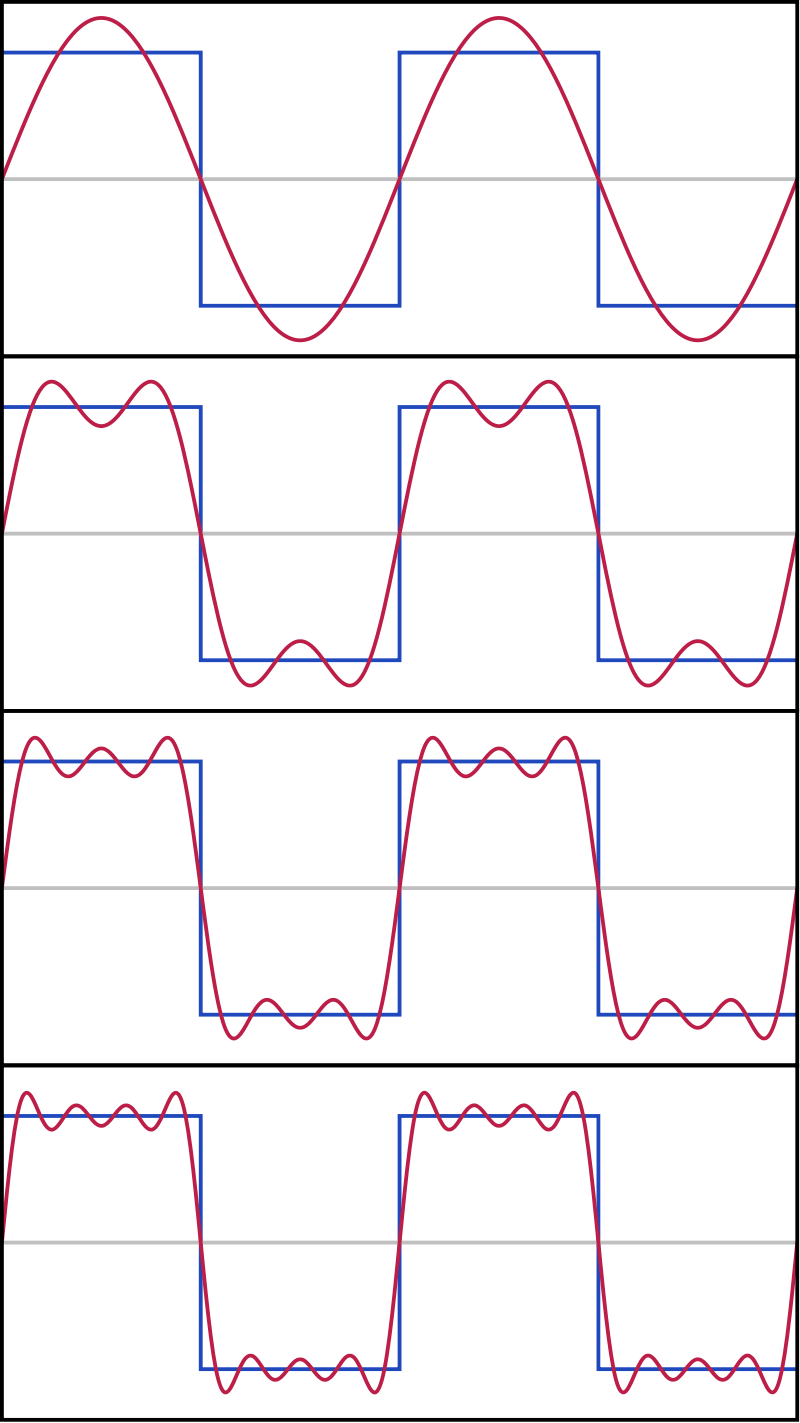
\includegraphics[width=.5\textwidth]{imagenes/imagenes20/T20IM12.png}
	\end{figure}
%\end{multicols}
\emph{Primeras cuatro aproximaciones para una función periódica escalonada}
\end{myblock}




 